\documentclass[a4paper]{article}
\title{\textcolor{red}{Workshop on Public Key Infrastructure and Red Hat Certificate System}}
\author{Niranjan M.R, Huzaifa Sidhpurwala, Asha Akkiangady}
\date{}
\usepackage{color}
\usepackage{graphics}
\usepackage{graphicx,subfig}
\begin{document}
\maketitle
\tableofcontents
\section{Introduction to Public Key Cryptography}
Before we start discussing about public key cryptography, we will in general discuss about how system communicate
and what are the various threat models that are associated with the communication medium and what are the tools to 
overcome them.

\textbf{Example1:}
The most common protocol used to communicate between 2 systems is TCP/IP. TCP/IP allows information to be sent 
from one system to another system directly or through many intermediate systems.

Below are some of the threat models associated with above communcation:
\begin{itemize}
    \item \textbf{Eavesdropping:}
        
        Information remains intact, But it's privacy is compromised, For example: some one could learn credit card number, record a sensitive conversation or intercept a
        classified information.
    \item \textbf{Tampering:}

        Information in transit is changed or replaced and then sent to the recipient. For example: Some one could alter an order of goods or change a persons resume.
    \item \textbf{Impersonation:}

        Information passes to a person who poses as intended recipient. Impersonation can take 2 forms:
    \begin{itemize}
        \item \textbf{Spoofing:}

            A person can pretend to be someone else, For example, a person can pretend to have email address \textit{joe@example.net}, 
            or computer can identify itself as a site called www.example.net, when it is not. This type of impersonation is called spoofing.
        \item \textbf{Misrepresentation:}

            A person or organization can misrepresent itself, For example, suppose the site \textit{www.example.net} pretends to be a 
            furniture store when it's just a site which accepts payments but never sends any goods.
    \end{itemize}
\end{itemize}
\textbf{Example2:}
Consider Alice , Bob and attacker are the parties , where alice and bob want to communicate to each other and Attacker is a threat to the communication.

\begin{itemize}
    \item Alice can send a postcard to bob to communicate, but this method is very weak as any random eavesdropper could read the postcard.
    \item Alice could write a letter and put in an envelope and send it to bob, but the attacker could open the envelope and read the letter, 
        both confidentiality and integrity of the message is lost.
    \item Alice could seal the envelope with wax , but this method too is inefficient as Attacker could read the letter and seal it as it is 
        without bob knowing that it was read by attacker
    \item Alice could write a letter and put it in a safe which has 2 keys and send one key before to Bob , and send the safe across to bob, 
        this ensures confidentiality, integrity but practically this is not implementable. Considering the number of 
        messages that has to be transferred , it's impractical to implement the mail safe method.
\end{itemize}

To mitigate above threat models, we will look in to cryptology as one of the tools of the trade. 

\textbf{Cryptology:} Cryptology is the theory of designing the various algorithms we use to provide security

\textbf{Cryptography:} Cryptography is the study of using these algorithms to secure systems and protocols.
\subsection{Encryption}
An encryption algorithm takes some data(called plaintext) and converts it to cipher-text under control of a key. 
cipher text contains random data which makes no sense without the key.  

A key is a short random string (8-24 bytes): 

\begin{picture}(10,10)(10,10)
    \put(40,1){\framebox(55,8){Plain Text}} 
    \put(102,10){\tiny Encryption}
    \put(102,4){\vector(1,0){30}}
    \put(140,1){\framebox(55,8){Cipher Text}} 
    \put(200,10){\tiny Decryption}
    \put(200,4){\vector(1,0){30}}
    \put(240,1){\framebox(55,8){Plain Text}} 
\end{picture}
\linebreak

When a message is encrypted and received , we cannot say if it's not tampered with. An encryption is strong when 
it can determine the number of possible keys. The attacker tries each key one at a time until he finds a key that 
produces a plausible decryption. The security of the algorithm should solely depend on the secrecy of the key. 
The algorithm should not need to be secret.

If the attacker knows the plaintext corresponding to the ciphertext it's called \textit{``known plaintext attack''} .

An attack where attacker doesn't know the plaintext , it's called \textit{``ciphertext-only attack''}.
\textit{Ex:} If the attacker knows that plaintext is ASCII , so any decryption which uses non-ascii characters must be using the wrong key.
\subsubsection{Symmetric Encryption}
When Sender and recipient share the same key(which must be kept secret) is referred to as \textit{Symmetric Key Cryptograph} or also
referred to as \textit{Secret Key Cryptography} as opposed to \textit{Public Key Cryptography}citation required?.
\begin{figure}[h]
    \centering
    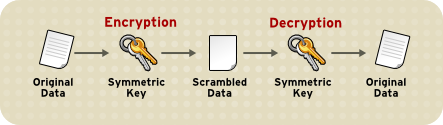
\includegraphics[width=50mm]{symmetric.png}
    \caption{Symmetric Encryption}
\end{figure}
\subsubsection{Assymetric Encryption}
\begin{itemize}
    \item First started in stanford university by Whitfield Diffie and Martin Hellman
    \item The most commonly used implementation of PKC are based on algorithm based on algorithm patented by RSA data security.
    \item Each public key is published \& private key is kept secret. Data encrypted with public key can be decrypted only with private key.
    \item In general, to send encrypted data to someone, we encrypt with public key \& the person encrypt receiving the 
        encrypted data decrypts with private key
    \item Compared to symmetric key encryption, public key encryption requires more computation \& therefore not always appropriate for large amounts of data
    \item It is possible to use public-key encryption to send a symmetric key, which can then be used to encrypt additional data.
        \begin{figure}[h]
            \centering
            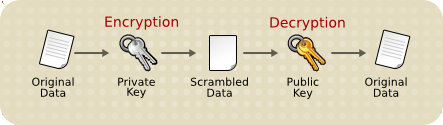
\includegraphics[width=80mm]{assymetric.png}
            \caption{Assymetric Encryption}
        \end{figure}
    \item Reverse of the above figure also happens i.e. encrypt with private key and decrypt with public-key. But not useful for sensitive information
        \begin{figure}[h]
        \centering
        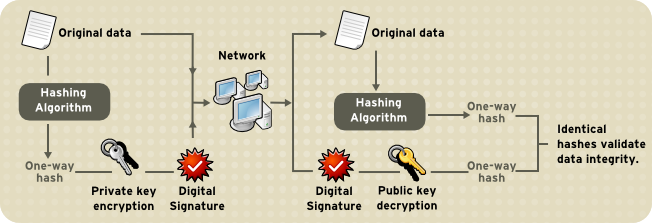
\includegraphics[width=80mm]{digitalsignature.png}
        \caption{Digital Signature}
        \end{figure}
    \item There's a problem with the above method, how would the parties get each other's public-key ? 
        If we send the keys through electronically, then the attacker an tamper, while they are in transit to the receiver.
    \item When the 2 parties want to communicate, the attacker can intercept the keys \& instead send his own key to each other, 
        thus each party encrypts to him and \& he re-encrypts it to the real recipient. 
        This is called \textit{man-in-the-middle attack}
        \begin{figure}[ht!]
            \centering
            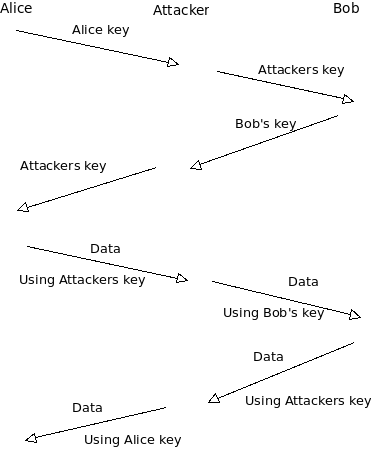
\includegraphics[width=50mm]{mitm.png}
            \caption{Man-in-the-middle attack}
        \end{figure}
\end{itemize}
\subsection{Message Digest}
A message digest is simply a function that takes as an input an arbitrary message and outputs a fixed length string 
which is characteristic of the message. The important property here is irreversibility.  
It's extremely difficult to compute a message from the given digest. 
Property of the message digest: 
\begin{itemize}
    \item For a digest to be secure, it must be difficult to generate any of the message that digests to the same value. 
        You have to search a message space of proportional size of the digest in order to find a matching message text
    \item It should be difficult to produce 2 messages M and M' such that they have the same digest. 
        This property is called collision-resistance. It turns out that the strength of any message digest 
        against finding collision is only half the size of the digest., so a 128-bit digest is only 64 bits strong against collisions.
\end{itemize}
\subsubsection{Message Authentication Code}
Consider \textit{Alice} and \textit{Bob} share a key and Alice wants to send a message to \textit{Bob}. The message can be encrypted, 
and send it across to \textit{Bob}, but we are not sure that the encrypted message would be tampered and also not sure 
if \textit{Alice} was the one who sent the encrypted message.  So we use a new tool called \textit{MAC} . \textit{MAC} is a digest algorithm,
but with a key, So the MAC is dependent on both the key and the message being MACed.
\subsection{Protocols}
\subsection{Exercises}
\section{Introduction to Public Key Infrastructure}
Below is a simplified architectural model of Public Key Infrastructure using X.509 (PKIX) Specifications
\begin{figure}[ht!]
    \centering
    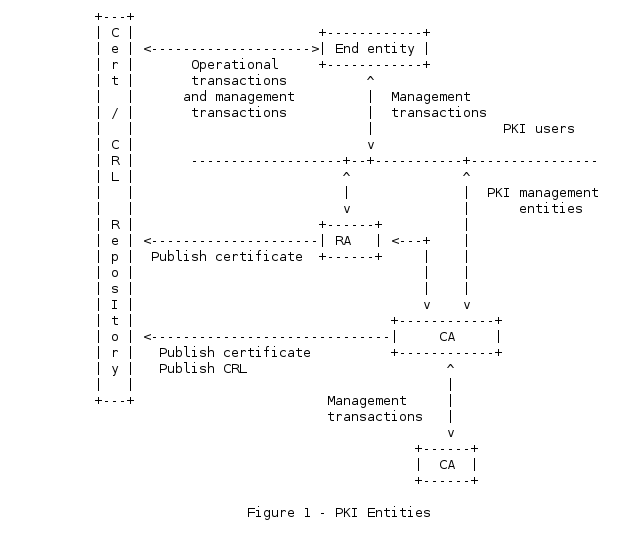
\includegraphics[width=70mm]{pki-architectural-model.png}
    \caption{PKI Architectural Model}
\end{figure}
\subsection{Common Terms used in PKI}
\begin{itemize}
    \item \underline{End Entiy}: User of the PKI certificates and/or end user system that is the subject of a certificate
    \item \underline{CA}: Certificate Authority
    \item \underline{RA}: Registration Authority, Optional System to which CA delegates certain management functions
    \item \underline{CRL issuers}: A system that generates CRL
    \item \underline{repository}: a system or collection of distributed systems that stores certificates and CRLs and services as a means of distributing these certificates and CRLs to end entities
\end{itemize}
\subsection{Detailed look on certificate/CRL}
    \subsubsection {Certificates}
        \begin{itemize}
            \item Certificates are data structures that bind public key values to the subject. This binding is asserted by a trusted Certificate Authority.
            \item X.509 defines the standard certificate format and v3 is the latest version.
            \item Internet Privacy Enhanced Mail(PEM) RFC 1421 and 1422 also include specifications for PKI based on X.509 certs. 
            \item Types of Certificates:
                \begin{itemize}
                    \item End-Entity
                    \item CA
                \end{itemize}
            \item RFC 1422 defines hierarchial structure  of CA's and there are three types of PEM CA
                \begin{itemize}
                    \item IPRA: Internet Policy Registration Authority , acts as Root of Certificate authority. IPRA operates under Internet Society Organization
                    \item PCA: Policy Certificae Authority ,(Verisign, Digicert, etc) signed by IPRA
                    \item CA: Certificate Authorities signed by PCA (Organizational CA's)
                \end{itemize}
            \item Policies used by CA:
                \begin{itemize}
                    \item IPRA certifies only PCA and not CA's or users cert
                    \item IPRA will make sure that the DN of the PCA is unique and will not certificate PCA's with similar DN
                    \item Certificates should not be issued to distinct entities under the same distinguished Name. 
                    \item IPRA should not certifiy two PCA's with same DN
                    \item PCA's should not certify two CA's with same DN
                    \item CA's are expected to sign certificates only if the subject DN in the
                        certificates is subordinate to the issuer CA DN.
                \end{itemize}
            \item Types of Certificate Authorities
                \begin{itemize}
                    \item Cross-Certs: Where Issuer and Subject are different
                    \item Self-Issue: Where Issuer and Subject are same
                        \begin{itemize}
                            \item Self-Signed: Where key bound in to the certificate is same as the key used to sgin the certificate
                        \end{itemize}
                \end{itemize}
        \end{itemize}
    \subsubsection{Revocation}
        When a certificate is issued, it is expected to be used for it's entire validity period. Due to various circumstances, certificate can be invalidated like:
        \begin{itemize}
            \item Change of name
            \item Change of association with subject and CA (Employee left)
            \item Compromise or private key
            \item CA wants to revoke the certificate
        \end{itemize}
        \begin{itemize}
            \item X.509 defines one method of revoking certificates, where CA periodically issues a signed data structure called Certificate revocation list (CRL).
            \item CRL is a time-stamped list identifying revoked certificates that is signed by CA or CRL issuer. 
            \item This list is freely available through public repositories
            \item It is expected that the certificate system user not only verifies certificate validity, signature but also aquires latest CRL from public repositories and check against CRL
            \item CRL's are issued periodically (hourly, daily or weekly). 
        \end{itemize}
    \subsubsection{Basic Certificate Fileds}
        \begin{itemize}
            \item Version:
                \begin{itemize}
                    \item Describes the version of encoded certificate.
                    \item if extensions are used: \textbf{0x2(3)}
                    \item if extensions are not used but UniqueIdentifier is used: \textbf{0x1(2)}
                    \item if only basic fields are there: \textbf{0x0(1)}
                \end{itemize}
                \begin{itemize}
                    \item Values: \textbf{0x2(3), 0x1(2), 0x0(1)}
                \end{itemize}
            \item Serial Number:
                \begin{itemize}
                    \item Positive integer assigned by CA to each certificate
                    \item It must be unique for each Certificate given by CA
                    \item Can contain long integers (up to 20 Octets)
                \end{itemize}
                \begin{itemize}
                    \item Values: Integers: 
                    \begin{itemize}
                        \item \textbf{16694152257348400000}
                        \item \textbf{0xe7ad8b07558a1727}
                        \item \textbf{cd:ba:7f:56:f0:df:e4:bc:54:fe:22:ac:b3:72:aa:55}
                    \end{itemize}
                \end{itemize}
            \item Signature:
                \begin{itemize}
                    \item Algorithm used by \textbf{CA} to sign the certificate
                    \item Value:
                        \begin{itemize}
                            \item \textbf{md2WithRSAEncryption}
                            \item \textbf{sha1WithRSAEncryption}
                        \end{itemize}
                \end{itemize}
            \item Issuer:
                \begin{itemize}
                    \item Identifies the entity that has signed and issued the certificate
                    \item \textbf{MUST} contain non-empty Distinguished Names
                    \item Names should confirm to X.501 standard
                    \item Generally contains Country, Organization, Common name, SerialNumber,
                        province, State, title, Surname, Generation Qualifier(Jr, Sr).
                    \item Values:
                    \begin{itemize}
                        \item \textbf{C=US, O=VeriSign, Inc., OU=Class 1 Public Primary Certification Authority}
                        \item \textbf{C=DE, ST=Bayern, L=Muenchen, O=Whatever it is, CN=IO::Socket::SSL Demo CA}
                        \item \textbf{C=US, O=VeriSign, Inc., OU=Class 1 Public Primary Certification Authority}
                    \end{itemize}
                \end{itemize}
            \item Validity:
                \begin{itemize}
                    \item The time interval during which the CA warrants that it will maintain status of the certificate
                    \item Consists sequence of 2 dates
                        \begin{itemize}
                            \item Date on which certificate validity begins
                            \item Date on which certificate validity ends
                        \end{itemize}
                    \item Validity period of a certificate is period from notBefore to notAfter(inclusive)
                    \item Values:
                        \begin{itemize}
                            \item \textbf{Not Before: Jan 29 00:00:00 1996 GMT}
                            \item \textbf{Not After : Aug  1 23:59:59 2028 GMT}
                            \item Special Note:
                                \begin{itemize}
                                    \item Devices are given certificates where there is no expiration date
                                    \item Value:
                                    \item Certificate is to be used for entire lifetime of the device \textbf{ Not After: 99991231235959Z.(represented in Generalized Time)}
                                \end{itemize}
                        \end{itemize}
                    \end{itemize}
        \end{itemize}
\subsection{Exercises}
\section{Red Hat Certificate System}
\subsection{Certificate Manager}
\subsubsection{Introduction}
Certificate Manager is the first subsystem that needs to be configured in PKI Environment, Certificate Manager can be configured as RootCA, Subordinate CA
\subsubsection{Installation}
    \begin{itemize}
        \item RPM: \textrm{\textbf{pki-ca}}
        \item configuration:  CA subsystem is configured using utility \textbf{pkispawn}. 
            
            pkispawn provides both interactive configuration  or silent configuration by reading a configuration file. 
            
            pkispawn first reads \textbf{default.cfg} first and gets other deployment specific information through interactive method
            or through batch mode by reading a file. 

            pkispawn then passes this information to a java servlet which performs the configuration. 
        \begin{figure}[ht!]
            \centering
            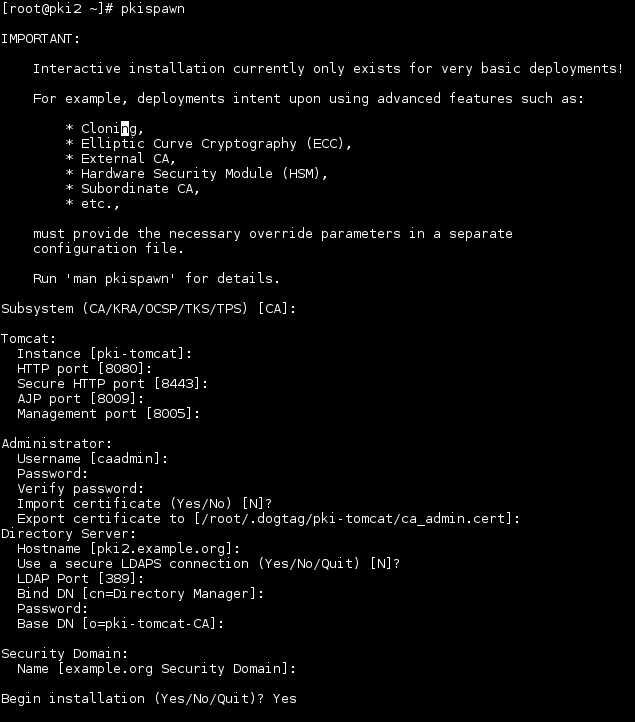
\includegraphics[width=90mm]{pkispawn-ca.png}
            \caption{Configuring CA subsystem using pkispawn}
        \end{figure}
    \end{itemize}
\subsubsection{Key Features}
    \begin{itemize}
        \item CA subsystem issues, renews, revokes Certificates, generates Certificat Revocation lists
        \item Publishes Certificates/CRL in form of files or can publish to LDAP or OCSP responder
        \item CA also has an inbuilt OCSP responder enabling OCSP-Compliant clients to query CA about revocation status of Certificate
        \item Some CA's can delegate some of it's responsibility to another Subordinate CA
    \end{itemize}
\subsubsection{Architecture}
     \begin{figure}[ht!]
          \centering
          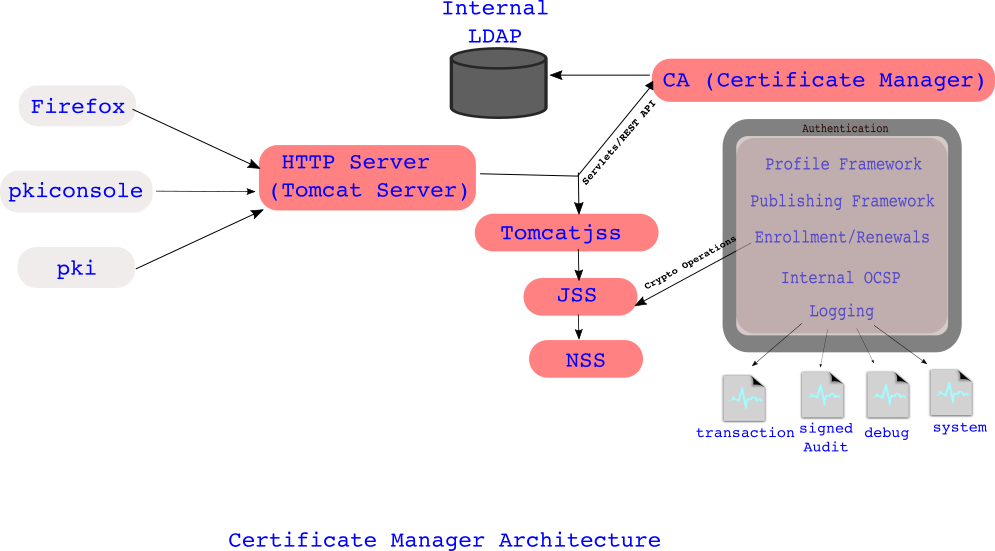
\includegraphics[width=120mm]{CA-subsystem-Arch3.png}
          \caption{CA Subsystem Architecture}
    \end{figure}
\subsubsection{Interfaces}
    \begin{itemize}
        \item End User Interface(Browser/CLI)
        \item Agent Interface(Browser/CLI)
        \item Admin interface(java console)
    \end{itemize}
\subsubsection{Features}
    \begin{itemize}
        \item Enrollment:

            End user Enrolls in the PKI infrastructure by submitting a Enrollment(certificate) request through End Entity Interface.
            This request can be submitted through 2 Methods:
            \begin{itemize}
                \item Browser
                \item CLI
            \end{itemize}
            There can be different kinds of Enrollment(Certificate) Request:
            \begin{itemize}
                \item Request for User, Server, SMIME, Dual Cert,.. certificate
                \item Request certificate if authentication through ldap, pin, cert etc. 
            \end{itemize}
            Based on the above types, there are different certificate profiles associated with it. 
            When end-entity(user) enrolls a certificate following events occur:
            \begin{itemize}
                \item The End-entity provides the information in one of the enrollment forms and submits a request
                \item The enrollment forms triggers the creation of public-key and private-key or dual-key pairs
                \item The End-entity provides authentication credentials before submitting the request,
                     depending on the authentication type. This can be LDAP authentication, PIN-based authentication or certificate-based authentication.
                \item The request is submitted either to an agent-approved enrollment process or an automated process.
                    \begin{itemize}
                        \item Agent-approved process requires no end-entity authentication, sends the request to the request queue in the agent-services interface.
                        \item Automatic notification can be setup so an email can be sent to an agent any time a request appears in the queue
                        \item The automated process, which involves end-entity authentication,process the certificate as soon as the end-entity successfully authenticates
                    \end{itemize}
                \item This form collects information about the end entity from the LDAP directory when the form is submitted
                \item The profile associated with form determine the aspects of certificate that is issued. Depending upon the certificate profile the request is evaluated to determine if the request meets the constraints set.
                \item The Certificate request is either rejected because it did not meet the certificate profile or authentication requirement, or a certificate is issued
                \item The certificate is delivered to end-entity  through HTML interface or email or certificate can be retrieved through Agents interface by serial number or request-ID.
                \item The new certificate is stored in Certificate Managers internal database.
                    \begin{figure}[ht!]
                    \centering
                    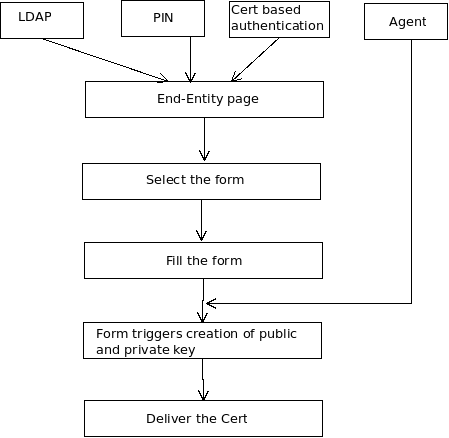
\includegraphics[width=35mm]{enrollment.png}
                    \caption{Certificate Enrollment}
                    \end{figure}
                \end{itemize}
        \item Profiles:

            Profile determine the content of a certificate. Certificate manager provides customizable framework to apply 
            policies for incoming certificate requests and to control the input requests types and output certificate types

            Certificate Profile define the following:
            \begin{itemize}
                \item  Authentication Method
                \item  Authorization Method
                \item  Certificate content
                \item  Constraints for the values of content
                \item  Contents of input
                \item  Output
            \end{itemize}
            \begin{figure}[ht!]
                \centering
                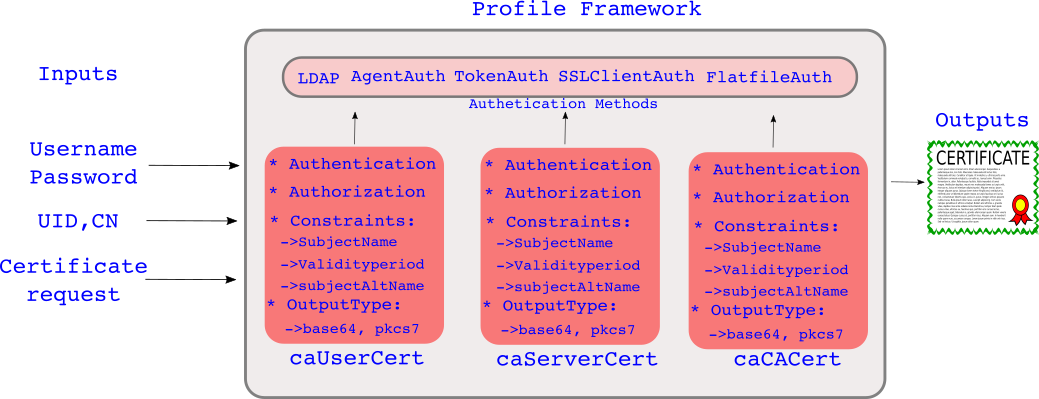
\includegraphics[width=90mm]{CA-profiles-arch.png}
                \caption{Certificate Profile Architecture}
            \end{figure}
            Profile Workflow:
            \begin{figure}[ht!]
                \centering
                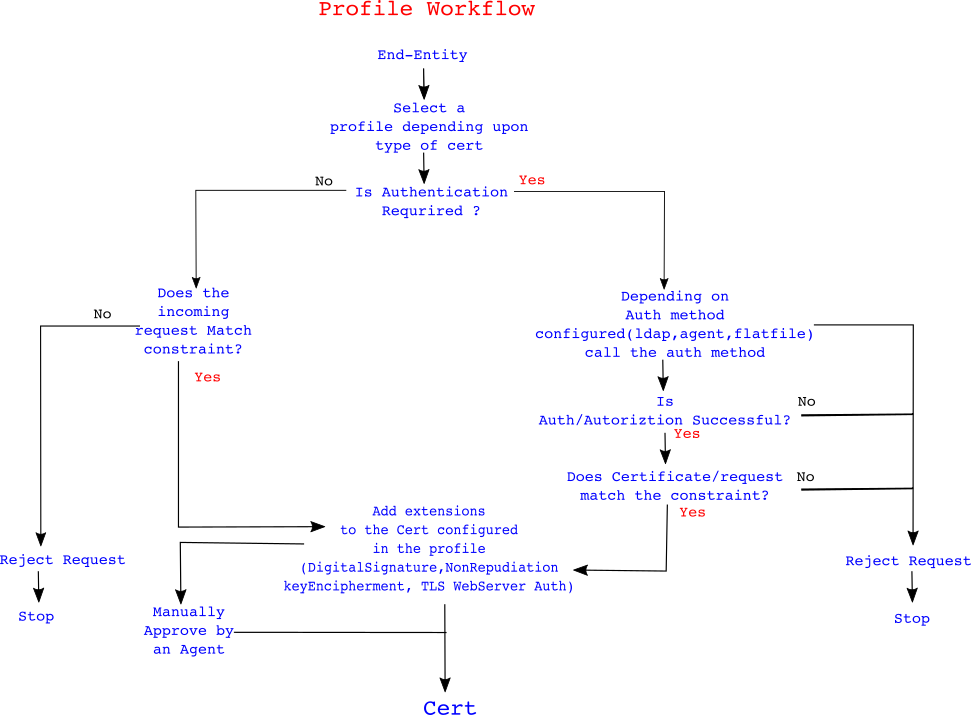
\includegraphics[width=80mm]{CA-Profiles-workflow.png}
                \caption{Certificate Profiles Workflow}
            \end{figure}
            
            Each profile are defined in \textbf{.cfg} file located at \textbf{/var/lib/instance\_name/profiles/ca} directory

            Example \textbf{caUserCert} Profile:

            The first part of the profile is the description and specifies whether profile is enabled or disabled, if enabled who
            enabled it. 
            \begin{figure}[ht!]
                \centering
                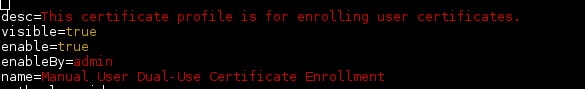
\includegraphics[width=80mm]{profile-1.png}
                \caption{Profile Description}
            \end{figure}
            
            The second part of the profile describes the inputs:
            \begin{figure}[ht!]
                \centering
                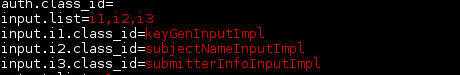
\includegraphics[width=80mm]{profile-2.png}
                \caption{Profile inputs}
            \end{figure}
            \begin{itemize}
                \item \underline{KeyGenInputImpl}: specifies the key pair generation during the request submission, This provides if the request
                    should be of type CRMF/PKCS10, also provides dropdown specifying the key size.
                \item \underline{subjectNameInputImpl}: specifies the subject Distinguished Name(DN) to be used in the cert. The subject DN 
                    can be constructed from \textit{UID, Email, Common Name, Organizational Unit, Country}
                \item \underline{submitterInfoImpl}: This input specifies three fields: \textit{Requester Name, Requester email, Requester phone}
            \end{itemize}
            \begin{figure}[ht!]
                \centering
                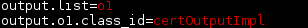
\includegraphics[width=80mm]{profile-3.png}
                \caption{Profile output}
            \end{figure}
            Third part of the profile is output, 
            \begin{itemize}
                \item \underline{certOutputImpl}: The certificate output format \textit{base64, pkcs7, prettyprint}
            \end{itemize}
            \begin{figure}[ht!]
                \centering
                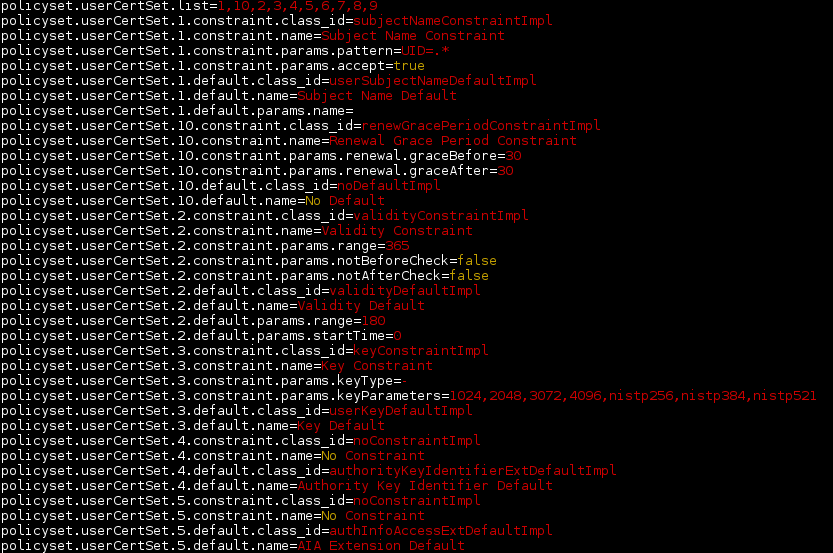
\includegraphics[width=80mm]{profile-4.png}
                \caption{Profile Policies}
            \end{figure}

            Last part of the profile is constraints, Policies like:
            \begin{itemize}
                \item validity of the cert
                \item renewal settings, 
                \item key Usage Extensions
                \item User supplied extensions
            \end{itemize}
        \item Publishing 
            Certificate System provides customizable framework from CA's to publish.
            \begin{figure}[h!]
                \centering
                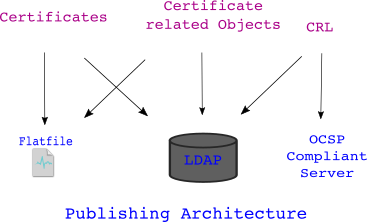
\includegraphics[width=40mm]{publishing3.png}
                \caption{Publishing Architecture}
            \end{figure}
            \begin{itemize}
                \item Key Features
                    \begin{itemize}
                        \item Publish to a single repositories or multiple repositories
                        \item Split locations by certificates/CRL
                        \item Set individual rules for each type of certs/crl
                    \end{itemize}
                \item Publishing framework consists
                    \begin{itemize}
                        \item Publishers
                        \item Mappers
                        \item Rules
                    \end{itemize}
                \item \underline{Publishers:}
                    Publishers specify location to which certificates/CRL's are to be published. 
                        Example: 
                        \begin{itemize}
                            \item To publish to a file, publishers specify the location of the publishing directory.
                            \item To publish to LDAP, publishers specify the attribute in the directory that srores the cert/CRL.
                            \item To publish to OCSP, we specify OCSP Server details. 
                        \end{itemize}
                    \item \underline{Rules}: Rules define 
                        \begin{itemize}
                            \item what is to be published and where ?
                            \item What type of certs can be published to what location
                            \item Set rules to publish certs to file and LDAP
                            \item Set individual rules for each type of cert/rule
                            \item There are rules for Files, LDAP and OCSP
                        \end{itemize}
                    \item \underline{Mappers}: Mappers are only used when publishing to LDAP
                        \begin{itemize}
                            \item Mappers construct the DN for an entry based on the information
                                from the certificate or certificate request. 
                            \item Mappers use certificate or certificate request's subject name to
                                construct the DN of the entry to which cert/certificate request/CRL has to be published
                        \end{itemize}
            \end{itemize}
    \end{itemize}
\subsubsection{Exercises}
\subsection{Key Recovery Authority}
\subsection{Online Certificate Status Protocol}
\subsection{Token Key Service \& Token Processing System}
\end{document} 
